%\newpage
\section{Ergebnisse und Berechnungen}
\label{sec:ergebnisse}


\begin{table}[h!]
		\centering
	\rowcolors{2}{gray!25}{white}
	\caption{Temperatur- und Druckmesswerte für die Reihenschaltung}
	%\resizebox{14cm}{!}{
	\begin{tabulary}{\textwidth}{L|C|C}
		\textbf{Messstelle} & \textbf{Temperatur} $\left[\si{\celsius}\right]$& \textbf{Druck} $\left[\si{\bar}\right]$\\
		\hline
		$T_{\alpha,\text{warm}}$ & 55,38 & 1,030\\
		$T_{\text{zw1},\text{warm}}$  & 46,58 & 0,690  \\
		$T_{\text{zw2},\text{warm}}$  & 46,56 & 0,500\\
		$T_{\omega,\text{warm}}$  & 32,73 & 0,215 \\
		\hline
		$T_{\alpha,\text{kalt}}$  & 16,10 & 2,300\\
		$T_{\text{zw2},\text{kalt}}$   & 36,71 & 0,900  \\
		$T_{\text{zw1},\text{kalt}}$   & 36,75 & 1,300   \\
		$T_{\omega,\text{kalt}}$ & 49,68 & 0,065 \\
	\end{tabulary}%
%}
	\label{tab:messung_reihe}%
\end{table}%
\FloatBarrier
\,

% Table generated by Excel2LaTeX from sheet 'Daten'
\begin{table}[h!]
	\renewcommand*{\arraystretch}{1.2}
	\centering
	\rowcolors{2}{gray!25}{white}
	\caption{Strömungsrelevante Größen der Reihenschaltung}
	\label{tab:strom_reihe}
	\resizebox{15cm}{!}{
		\begin{tabulary}{1.2\textwidth}{CCCCC}
			\hline
			\textbf{Strom}&\textbf{Fläche} $\left[\si{\sqm}\right]$&\textbf{hydr. Durchmesser} $\left[\si{\meter}\right]$&\textbf{Volumenstrom} $\left[\si{\cmt\per\second}\right]$&\textbf{Geschwindigkeit} $\left[\si{\meter\per\second}\right]$ \\
			\hline
			warm&\SI{7,85E-05}{}&\SI{0,01}{}&\SI{1,32E-04}{}&\SI{1,68}{}\\
			kalt	&\SI{6,83E-05}{}&\SI{0,003}{}&\SI{8,63E-05}{}&\SI{1,26}{}\\
			\hline			
	\end{tabulary}
}
\end{table}%
\FloatBarrier

% Table generated by Excel2LaTeX from sheet 'GegenstromReihe neu'
\begin{table}[h!]
	\renewcommand*{\arraystretch}{1.2}
	\centering
	\rowcolors{2}{white}{gray!25}
	\caption{Berechnete Wärmeströme und Korrekturvolumenstrom für die Reihenschaltung}
	\resizebox{15cm}{!}{
	\begin{tabulary}{1.2\textwidth}{C|CC|C|CC|C}
		\hline
		\textbf{System} & $\boldsymbol{Q_{ab}} \, \left[\si{\kilo \watt}\right]$ & $\boldsymbol{Q_{auf}} \, \left[\si{\kilo \watt}\right]$& $\boldsymbol{\dot{V}_{korr}} \, \left[\si{\cmt \per \second}\right]$& $\boldsymbol{Q_{ab, korr}} \, \left[\si{\kilo \watt}\right]$&$\boldsymbol{Q_{auf, korr}} \, \left[\si{\kilo \watt}\right]$ & $\boldsymbol{\Delta Q_{korr}} \, \left[\si{\kilo \watt}\right]$\\
		\hline
		WÜ1   & 7,58  & 7,44  &\SI{ -9,70E-07 }{}& 7,53  & 7,53  & 0,00 \\
		WÜ2   & 4,83  & 4,67  & \SI{-1,71E-06}{} & 4,76  & 4,76  & 0,00 \\
		\hline
		Gesamt & 12,42 & 12,13 & \SI{-1,24E-06}{} & 12,30 & 12,30 & 0,00 \\
		\end{tabulary}%
	}
	\label{tab:warme_reihe}%
\end{table}%
\FloatBarrier
\,
\begin{table}[h!]
	\centering
	\rowcolors{2}{gray!25}{white}
	\caption{Berechnete Leistungen, dimensionslose Kennzahlen und Wärmeübertragungsparameter der Reihenschaltung}
	\resizebox{15cm}{!}{
	\begin{tabulary}{1.5\textwidth}{L|C|CCC|CCC|CC}
		\hline
		\textbf{System} & $\boldsymbol{\Delta p} \, \left[\si{\bar}\right]$ & $\boldsymbol{P_{Pumpe}} \, \left[\si{\kilo \watt}\right]$ &  $\boldsymbol{P_{Elektrisch}} \, \left[\si{\kilo \watt}\right]$& $\boldsymbol{Q/P_{Elektrisch}}$ & \textbf{Re} & \textbf{Pr}& \textbf{Nu} & $\boldsymbol{\alpha}  \, \left[\si{\kilo \watt \per \sqm \per \kelvin}\right]$ & $\boldsymbol{U} \, \left[\si{\kilo \watt \per \meter\per \kelvin}\right]$ \\
		\hline
		Gesamt warm & 0,82  & \SI{1,07E-02}{} & \SI{1,34E-02}{} & 916   & -&- & -& - & -\\
		Gesamt kalt & 2,24  & \SI{1,93E-02 }{}& \SI{2,41E-02}{} & 510   & - & - & - & -& -\\
		\hline
		WÜ1 warm & 0,29  & \SI{3,76E-03}{} & \SI{4,70E-0}{}3 & 1602  & \SI{2,20E+04}{} & 5,13  & \SI{1,32E+02}{} & 8,14  & 0,0311 \\
		WÜ1 kalt & 20,61 &\SI{ 1,78E-01 }{}&\SI{ 2,22E-01}{} & 34    &\SI{ 3,41E+03}{} & 7,87  & \SI{3,52E+01 }{}& 6,93  &  \\
		\hline
		WÜ2 warm & 0,35  & \SI{4,66E-03 }{}& \SI{5,83E-03 }{}& 817   & \SI{2,87E+04}{} & 3,80  & \SI{1,45E+02}{} & 9,20  & 0,0350 \\
		WÜ2 kalt & 12,93 & \SI{1,12E-01}{} &\SI{ 1,40E-01 }{}& 34    & \SI{5,39E+03}{} & 4,68  & \SI{4,12E+01}{} & 8,57  &  \\
	\end{tabulary}%
}
	\label{tab:leistung_reihe}
\end{table}%




Um die verschiedenen Wärmetauscher vergleichen zu können und ein Optimum für den Betrieb des Wärmetauschers zu verfolgen, wird eine Linearisierung der \textsc{Nußelt}-Gleichung mit den Parametern $a$ und $b$ vorgenommen (siehe Gl.\eqref{gl:linearisierung}).
Diese werden für die verschiedenen Versuchsbedingungen und Wärmetauscher im Diagramm Abb. \ref{dia:nusselt} aufgetragen.

\begin{flalign}
\label{gl:linearisierung}
\tag{Geradengleichung} y 	&= m*x + n\\
\tag{logarithmieren}
Nu 	&= a*\left(Re^2*Pr\right)^b\\
\ln(Nu) 	&= \ln(a)+b*\ln(Re^2*Pr)
\end{flalign}

\begin{figure}[h!]
		\begin{center}
			\resizebox{0.8\textwidth}{!}{
				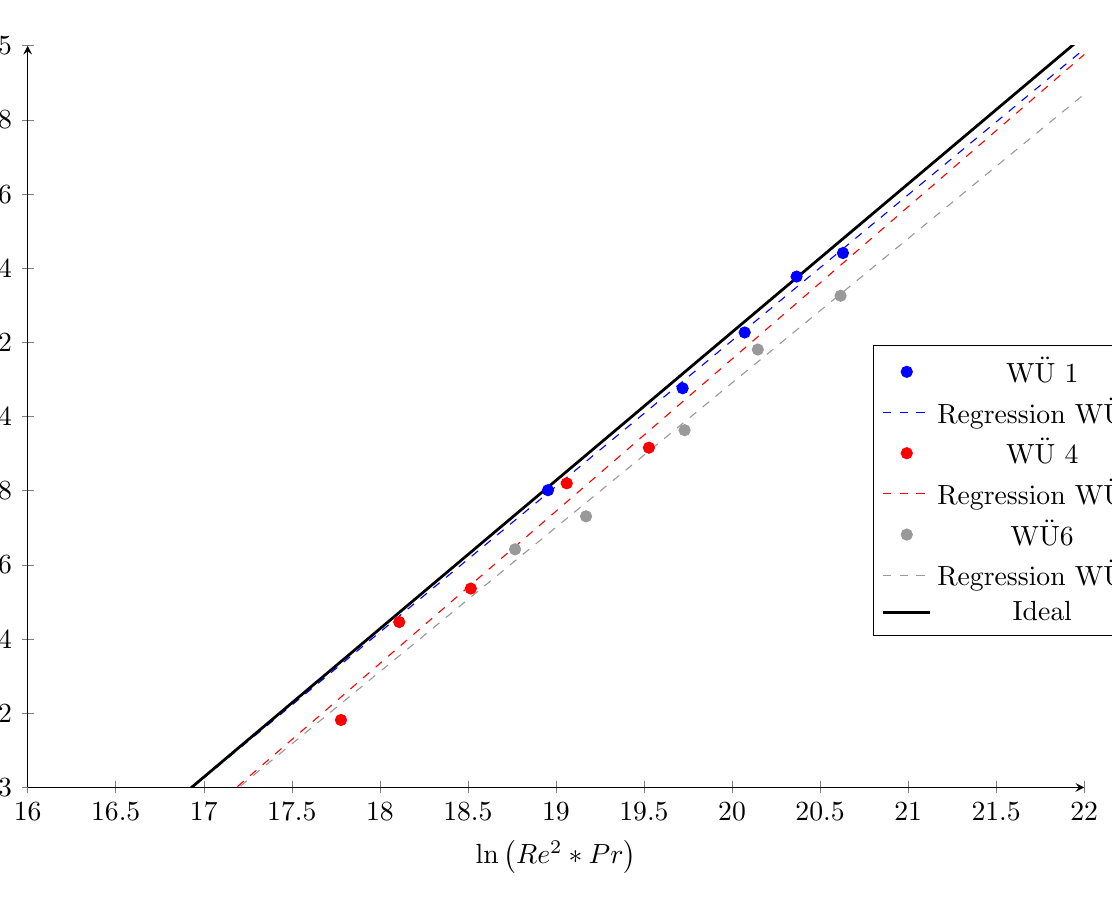
\begin{tikzpicture}[trim axis left, trim axis right]
				\begin{axis}[
				axis lines = left,
				width = 15cm,
				height = 11cm,
				xmin = 16,
				xmax = 22,
				ymin = 3,
				ymax = 5,
				%	ytick = {-4.5,-4,...,-1},
				%	xtick = {-10,-9,...,20},
				ylabel={$\ln(Nu)=\ln(a)$},
				%y label style={at={(0,0.5)}},
				xlabel={$\ln\left(Re^2*Pr\right)$},
				legend style={at={(0.8,0.4)},anchor=west},
				%	y dir = reverse,
				]
				\addplot [color=blue, mark=*, only marks] coordinates{(20.6297374908074,4.44104369234906) (18.9546273718935,3.80144109711371) (20.0716652877696,4.22683350226042) (20.3663656925989,4.37753401861674) (19.7192916621653,4.07642094111326) };
				
				\addplot +[mark=none, dashed, blue, domain=0:25] {x*0.393184906-3.658730546};
				
				
				\addplot [color=red, mark=*, only marks] coordinates{(19.5277930158006,3.91608551420758) (19.0610517373774,3.82007146704219) (18.5164491828898,3.53620711030527) (18.1099284493333,3.44591529294571) (17.7790640575647,3.18172509942449) };
				
				\addplot +[mark=none, dashed, red, domain=0:25] {x*0.410555238-4.055857385};
				
				\addplot [color=black!40!white, mark=*, only marks] coordinates{(20.6162086982967,4.32579265627852) (20.1461082909801,4.18077187238098) (19.7303635113762,3.9632873963571) (19.1706257554954,3.73097328400248) (18.7674483798004,3.64195918704045)  };
				
				\addplot +[mark=none, dashed, color=black!40!white, domain=0:25] {x*0.389412718-3.697480663};
								
				\addplot [color=black, mark=none,line width=1.pt ] coordinates{	(10,0.227738936947013) (10.5,0.427738936947013) (11,0.627738936947013) (11.5,0.827738936947013) (12,1.02773893694701) (12.5,1.22773893694701) (13,1.42773893694701) (13.5,1.62773893694701) (14,1.82773893694701) (14.5,2.02773893694701) (15,2.22773893694701) (15.5,2.42773893694701) (16,2.62773893694701) (16.5,2.82773893694701) (17,3.02773893694701) (17.5,3.22773893694701) (18,3.42773893694701) (18.5,3.62773893694701) (19,3.82773893694701) (19.5,4.02773893694701) (20,4.22773893694701) (20.5,4.42773893694701) (21,4.62773893694701) (21.5,4.82773893694701) (22,5.02773893694701) (22.5,5.22773893694701) (23,5.42773893694701) (23.5,5.62773893694701) (24,5.82773893694701) (24.5,6.02773893694701) (25,6.22773893694701) (25.5,6.42773893694701) (26,6.62773893694701) (26.5,6.82773893694701) (27,7.02773893694701) (27.5,7.22773893694701) (28,7.42773893694701)  };
				
				\legend{WÜ 1, Regression WÜ 1, WÜ 4, Regression WÜ 4, WÜ6, Regression WÜ 6, Ideal}
				\end{axis}
				\end{tikzpicture}
			}
			\caption{linearisierte \textsc{Nußelt}-Gleichung in Abhängigkeit von $Re$, $Pr$, $a$ und $b$}
			\label{dia:nusselt}
		\end{center}
	\end{figure}
	\FloatBarrier

Das Bestimmtheitsmaß Daten in Tab. \ref{tab:ab} gibt an, dass $R^2$ zwischen $0,827$ und $0,968$ liegt. Dadurch sind starke Abweichungen zu erkennen, die im Präsenspraktikum zumindest für WÜ 6 wiederholt werden sollte.
Ansonsten lässt sich aus Abb. \ref{dia:nusselt} erkennen, dass die Regressionsgeraden von WÜ 1 am nächsten an der idealen Geraden anliegt.
